% Outil GRC -- Documentation technique
% Compile with:  latexmk -xelatex GRC_Tool_Documentation.tex
\documentclass[11pt,a4paper]{article}

\usepackage{fontspec}            % Latin Modern (default LaTeX look)
\usepackage{polyglossia}
\setmainlanguage[autospacing=false]{french}
\providecommand{\og}{«~}\providecommand{\fg}{~»}
\usepackage[a4paper,margin=2.5cm,headheight=14pt]{geometry}
\usepackage{microtype}
\usepackage{graphicx}
\usepackage{booktabs,tabularx,array,multirow}
\usepackage[table]{xcolor}
\usepackage{tikz}
\usetikzlibrary{positioning,arrows.meta,shapes.multipart}
\usepackage{pgfplots}
\pgfplotsset{compat=1.17}
\usepackage{listings}
\usepackage{caption}
\usepackage{float}
\usepackage{enumitem}
\usepackage{fancyhdr}
\usepackage{titlesec}
\usepackage[most]{tcolorbox}
\usepackage{amsmath}
\usepackage[hidelinks]{hyperref}

\graphicspath{{../screenshots/}}

% ---------- colours ----------
\definecolor{navy}{HTML}{0F2A47}
\definecolor{accent}{HTML}{1F5F99}
\definecolor{lightbg}{HTML}{F4F6F8}
\definecolor{rcrit}{HTML}{C0392B}
\definecolor{rhigh}{HTML}{E67E22}
\definecolor{rmed}{HTML}{F1C40F}
\definecolor{rlow}{HTML}{27AE60}

\hypersetup{pdftitle={Outil GRC -- Documentation technique},pdfauthor={Douae Admi}}

\titleformat{\section}{\Large\bfseries\color{navy}}{\thesection}{1em}{}
\titleformat{\subsection}{\large\bfseries\color{accent}}{\thesubsection}{1em}{}

\pagestyle{fancy}\fancyhf{}
\fancyhead[L]{\small\textsc{Outil GRC}}
\fancyhead[R]{\small\nouppercase{\leftmark}}
\fancyfoot[C]{\small\thepage}
\renewcommand{\headrulewidth}{0.4pt}

\captionsetup{font=small,labelfont=bf}
\setlength{\emergencystretch}{3em}
\setlist{itemsep=2pt}

\lstset{basicstyle=\ttfamily\small,backgroundcolor=\color{lightbg},frame=single,
  rulecolor=\color{black!15},keywordstyle=\color{accent}\bfseries,commentstyle=\color{black!50}\itshape,
  stringstyle=\color{rcrit!80!black},showstringspaces=false,breaklines=true,
  xleftmargin=4pt,xrightmargin=4pt,aboveskip=8pt,belowskip=8pt,extendedchars=true}

\newtcolorbox{keybox}[1][]{colback=accent!6,colframe=accent,boxrule=0.6pt,arc=2pt,
  left=6pt,right=6pt,top=4pt,bottom=4pt,fonttitle=\bfseries,#1}

\newcommand{\code}[1]{\texttt{#1}}
\newcommand{\lvl}[2]{\textcolor{#1}{\textbf{#2}}}

\begin{document}

% ================= PAGE DE TITRE =================
\begin{titlepage}
\centering
\vspace*{2.5cm}
{\scshape\large Documentation technique\par}
\vspace{1.2cm}
\rule{\linewidth}{0.8pt}\par\vspace{0.4cm}
{\Huge\bfseries Outil GRC\par}
\vspace{0.4cm}
{\Large Suivi de la conformité ISO/IEC 27001:2022 \& DNSSI\\ et registre des risques\par}
\vspace{0.3cm}
\rule{\linewidth}{0.8pt}\par
\vspace{1cm}
{\large Application web Django --- cas d'étude : \emph{AtlasPay}, fintech marocaine fictive\par}
\vfill
{\Large Douae \textsc{Admi}\par}
\vspace{0.2cm}
{Élève ingénieure en cybersécurité\par}
\href{https://github.com/Dorvae}{\texttt{github.com/Dorvae}}\par
\vspace{1.5cm}
{\small Python $\cdot$ Django 6.0 $\cdot$ SQLite \hfill Version 1.2 --- novembre 2026\par}
\end{titlepage}

\tableofcontents
\newpage

% ================= 1 =================
\section{Synthèse}
Ce document présente la conception, la réalisation et les résultats d'une application web de \textbf{Gouvernance, Risques et Conformité (GRC)} développée avec le framework Django. L'outil tient un catalogue de contrôles de sécurité, enregistre le niveau de conformité de l'organisation pour chaque contrôle, calcule un \textbf{taux de conformité par domaine} et maintient un \textbf{registre des risques} dans lequel chaque risque est évalué et relié aux contrôles qui le traitent.

Deux référentiels sont couverts : la norme internationale \textbf{ISO/IEC 27001:2022} (annexe~A, organisée en quatre thèmes) et la \textbf{DNSSI} marocaine (\emph{Directive Nationale de la Sécurité des Systèmes d'Information}). L'outil a été appliqué à \textbf{AtlasPay}, une fintech de paiement fictive ; les évaluations ont été saisies les 27 et 28 juillet 2026.

\begin{table}[H]
\centering
\begin{tabularx}{\linewidth}{@{}lX@{}}
\toprule
\textbf{Élément} & \textbf{Résultat}\\
\midrule
Référentiels & ISO/IEC 27001:2022 (4 thèmes) + DNSSI\\
Catalogue & 5 domaines, 8 contrôles, 8 évaluations, 3 risques\\
Domaine le plus faible & Technologique --- \textbf{0\,\%} (authentification et cryptographie non conformes)\\
Domaines les plus solides & Personnes et Physique --- 50\,\%\\
Registre des risques & 2 risques \lvl{rcrit}{critiques}, 1 risque \lvl{rhigh}{élevé}\\
Livrables & Application Django, back-office d'administration, dashboard, formulaires de saisie, tests, jeu de données de démonstration\\
\bottomrule
\end{tabularx}
\caption{Chiffres clés}
\end{table}

\begin{keybox}[title=Constat principal]
Chaque risque du registre est relié à au moins un contrôle non conforme ou partiellement conforme. Les deux risques critiques reposent sur des contrôles technologiques (A.8.5 Authentification sécurisée, A.8.24 Utilisation de la cryptographie) tous deux évalués \emph{non conformes} : ce sont les premières priorités de remédiation.
\end{keybox}

% ================= 2 =================
\section{Contexte et objectifs}
\subsection{Contexte}
Les organisations des secteurs réglementés, comme les services de paiement, doivent démontrer que leurs contrôles de sécurité de l'information sont en place et efficaces. Ce suivi se fait souvent dans des tableurs dispersés, ce qui rend difficile la lecture du niveau global de conformité, le suivi des progrès entre deux audits, ou le lien entre un écart et le risque métier qu'il crée.

Au Maroc, les entités d'importance vitale et les infrastructures critiques sont en outre soumises à la DNSSI publiée par la DGSSI, qui ajoute à la base ISO~27001 des exigences organisationnelles (par exemple un responsable de la sécurité indépendant de l'exploitation informatique) et des exigences de souveraineté des données.

\subsection{Objectifs}
\begin{itemize}
  \item \textbf{Centraliser} le catalogue de contrôles ISO 27001:2022 et DNSSI dans une base de données unique.
  \item \textbf{Évaluer} chaque contrôle avec un statut normalisé et conserver un enregistrement daté et commenté.
  \item \textbf{Mesurer} automatiquement la conformité par domaine selon une règle de pondération transparente.
  \item \textbf{Recenser les risques} avec un score probabilité $\times$ impact et les relier aux contrôles qui les traitent.
  \item \textbf{Visualiser} la posture de sécurité sur un dashboard lisible par la direction.
\end{itemize}

\subsection{Périmètre du cas d'étude}
AtlasPay est une fintech fictive qui fournit des API de paiement aux commerçants, exploite une partie de son infrastructure en interne (on-premise) et traite des données personnelles et de paiement de ses clients. L'évaluation porte sur un sous-ensemble représentatif de huit contrôles plutôt que sur les 93 contrôles de l'annexe~A.

% ================= 3 =================
\section{Référentiels et catalogue de contrôles}
L'ISO/IEC 27001:2022 regroupe les 93 contrôles de son annexe~A en quatre thèmes : organisationnel (5.x), humain (6.x), physique (7.x) et technologique (8.x). L'outil utilise ces thèmes comme \emph{domaines} ; les exigences DNSSI forment un cinquième domaine.

\begin{table}[H]
\centering\small
\begin{tabularx}{\linewidth}{@{}lXll@{}}
\toprule
\textbf{Code} & \textbf{Contrôle} & \textbf{Domaine} & \textbf{Référentiel}\\
\midrule
A.5.9  & Inventaire des informations et autres actifs associés & Organisationnel & ISO 27001\\
A.5.19 & Sécurité de l'information dans les relations avec les fournisseurs & Organisationnel & ISO 27001\\
A.6.3  & Sensibilisation, enseignement et formation à la sécurité & Personnes & ISO 27001\\
A.7.1  & Périmètres de sécurité physique & Physique & ISO 27001\\
A.8.5  & Authentification sécurisée & Technologique & ISO 27001\\
A.8.24 & Utilisation de la cryptographie & Technologique & ISO 27001\\
RSSI   & Organisation de la sécurité --- séparation des fonctions DSI et RSSI & DNSSI & DNSSI\\
SOUV   & Souveraineté et hébergement des données & DNSSI & DNSSI\\
\bottomrule
\end{tabularx}
\caption{Catalogue de contrôles d'AtlasPay}
\end{table}

% ================= 4 =================
\section{Architecture de l'application}
L'outil suit le modèle \textbf{Modèle--Vue--Template (MVT)} de Django. Une seule application, \code{core}, porte la logique GRC ; le paquet projet, \code{grc\_project}, porte la configuration et le routage. Les données sont stockées dans SQLite, suffisant pour un outil mono-équipe et sans serveur de base de données.

\begin{figure}[H]
\centering
\begin{tikzpicture}[
  node distance=0.9cm and 1.1cm,
  comp/.style={draw=accent,fill=accent!8,rounded corners=3pt,minimum width=2.6cm,minimum height=1.1cm,align=center,font=\small},
  ext/.style={comp,fill=white},
  arr/.style={-{Stealth[length=2.2mm]},thick,black!60}]
\node[ext] (br) {\textbf{Navigateur}\\\scriptsize utilisateur / auditeur};
\node[comp,right=of br] (url) {\textbf{urls.py}\\\scriptsize routage};
\node[comp,right=of url] (vw) {\textbf{views.py}\\\scriptsize pages et formulaires};
\node[comp,right=of vw] (adm) {\textbf{Admin Django}\\\scriptsize back-office};
\node[comp,below=of url] (tpl) {\textbf{Templates}\\\scriptsize base + pages + CSS};
\node[comp,below=of vw] (frm) {\textbf{forms.py}\\\scriptsize ModelForms};
\node[comp,below=of frm] (mdl) {\textbf{models.py}\\\scriptsize logique métier};
\node[ext,right=of mdl] (db) {\textbf{SQLite}\\\scriptsize db.sqlite3};
\draw[arr] (br) -- node[above,font=\scriptsize]{HTTP} (url);
\draw[arr] (url) -- (vw);
\draw[arr] (vw) -- node[above left,font=\scriptsize]{rendu} (tpl);
\draw[arr] (vw) -- (frm);
\draw[arr] (frm) -- (mdl);
\draw[arr] (mdl) -- node[above,font=\scriptsize]{ORM} (db);
\draw[arr] (adm) -- (mdl);
\end{tikzpicture}
\caption{Flux d'une requête et composants}
\end{figure}

\begin{table}[H]
\centering\small
\begin{tabularx}{\linewidth}{@{}lX@{}}
\toprule
\textbf{Fichier} & \textbf{Rôle}\\
\midrule
\code{grc\_project/settings.py} & Configuration : applications, middlewares de sécurité (CSRF, sessions, clickjacking), base de données, templates\\
\code{grc\_project/urls.py} & Associe les cinq URL à l'admin et aux vues de \code{core}\\
\code{core/models.py} & Modèle de données et règles métier (taux de conformité, niveau de risque)\\
\code{core/views.py} & Accueil, dashboard, vues de création d'évaluations et de risques\\
\code{core/forms.py} & ModelForms générant des formulaires HTML validés\\
\code{core/admin.py} & Enregistre les quatre modèles dans l'admin Django\\
\code{core/templates/} & Gabarit \code{base.html} avec barre de navigation, étendu par chaque page\\
\code{core/static/core/style.css} & Code couleur des taux de conformité et des niveaux de risque\\
\bottomrule
\end{tabularx}
\caption{Composants}
\end{table}

\begin{table}[H]
\centering\small
\begin{tabular}{@{}lll@{}}
\toprule
\textbf{URL} & \textbf{Vue} & \textbf{Fonction}\\
\midrule
\code{/} & \code{home} & Page d'accueil\\
\code{/dashboard/} & \code{dashboard} & Conformité par domaine + registre des risques\\
\code{/evaluations/ajouter/} & \code{ajouter\_evaluation} & Saisir l'évaluation d'un contrôle\\
\code{/risques/ajouter/} & \code{ajouter\_risque} & Ajouter un risque et ses contrôles\\
\code{/admin/} & Admin Django & Back-office de toutes les entités\\
\bottomrule
\end{tabular}
\caption{Plan des URL}
\end{table}

Les deux vues de création suivent le modèle \emph{Post/Redirect/Get} : un POST valide enregistre l'objet puis redirige vers le dashboard, ce qui évite les doubles soumissions lors d'un rafraîchissement. Toutes les pages étendent un gabarit commun \code{base.html} qui fournit la barre de navigation.

% ================= 5 =================
\section{Modèle de données}
Un \textbf{Domaine} regroupe des \textbf{Contrôles} ; chaque contrôle reçoit une ou plusieurs \textbf{Évaluations} ; un \textbf{Risque} est relié aux contrôles qui le traitent par une relation plusieurs-à-plusieurs.

\begin{figure}[H]
\centering
\begin{tikzpicture}[
  ent/.style={rectangle split,rectangle split parts=2,draw=accent,thick,
    rectangle split part fill={navy,white},font=\small,text width=3.0cm,align=left,inner sep=4pt,anchor=north},
  rel/.style={thick,black!60}]
\node[ent] (dom) at (0,0) {\textcolor{white}{\textbf{Domaine}}\nodepart{second}id (PK)\\nom\\referentiel\\\textit{taux\_conformite()}};
\node[ent] (ctl) at (4.8,0) {\textcolor{white}{\textbf{Controle}}\nodepart{second}id (PK)\\code, libelle\\description\\domaine (FK)};
\node[ent] (ev) at (9.6,0) {\textcolor{white}{\textbf{Evaluation}}\nodepart{second}id (PK)\\controle (FK)\\statut (choix)\\date\_evaluation\\commentaire};
\node[ent] (rq) at (4.8,-3.4) {\textcolor{white}{\textbf{Risque}}\nodepart{second}id (PK)\\nom\\probabilite, impact\\\textit{niveau\_residuel()}};
\draw[rel] (dom.east) -- node[pos=0.12,above]{\small 1} node[pos=0.88,above]{\small N} (ctl.west);
\draw[rel] (ctl.east) -- node[pos=0.12,above]{\small 1} node[pos=0.88,above]{\small N} (ev.west);
\draw[rel,dashed] (ctl.south) -- node[pos=0.15,right]{\small M} node[pos=0.8,right]{\small N} node[midway,left,font=\scriptsize\itshape]{controles (M2M)} (rq.north);
\end{tikzpicture}
\caption{Diagramme entité--association}
\end{figure}

\begin{table}[H]
\centering\small
\begin{tabularx}{\linewidth}{@{}llX@{}}
\toprule
\textbf{Entité} & \textbf{Champs principaux} & \textbf{Remarques}\\
\midrule
Domaine & nom, referentiel & \code{taux\_conformite()} renvoie le taux, ou \code{None} si rien n'est évalué\\
Controle & code, libelle, domaine & Clé étrangère vers Domaine, suppression en cascade\\
Evaluation & controle, statut, date, commentaire & statut $\in$ \{conforme, partiel, non\_conforme, na\} ; date renseignée automatiquement\\
Risque & nom, probabilite, impact, controles & \code{niveau\_residuel()} classe $P\times I$ en quatre niveaux\\
\bottomrule
\end{tabularx}
\caption{Entités}
\end{table}

Stocker les évaluations comme des enregistrements distincts, plutôt que comme un champ du contrôle, conserve une \textbf{piste d'audit} : un contrôle peut être réévalué dans le temps et chaque évaluation garde sa date et son commentaire.

% ================= 6 =================
\section{Logique métier}
\subsection{Taux de conformité par domaine}
Chaque statut est converti en points ; les contrôles \emph{non applicables} sont exclus du numérateur et du dénominateur, comme dans une Déclaration d'Applicabilité (DdA) :
\[
\text{Taux}(d) \;=\; \frac{\displaystyle\sum_{e\,\in\,E_d} \text{pts}(e)}{|E_d|}\times 100,
\qquad
\text{pts}=\begin{cases}1 & \text{conforme}\\ 0{,}5 & \text{partiel}\\ 0 & \text{non conforme}\end{cases}
\]
où $E_d$ est l'ensemble des évaluations applicables du domaine $d$.

\begin{lstlisting}[language=Python]
def taux_conformite(self):
    points = {"conforme": 1, "partiel": 0.5, "non_conforme": 0}
    evaluations = Evaluation.objects.filter(
        controle__domaine=self
    ).exclude(statut="na")
    if not evaluations.exists():
        return None
    total_points = sum(points[e.statut] for e in evaluations)
    return round((total_points / evaluations.count()) * 100, 1)
\end{lstlisting}

\begin{keybox}[title=Exemple de calcul --- Organisationnel]
A.5.9 est \emph{partiel} (0,5) et A.5.19 est \emph{non conforme} (0) : $\text{Taux} = \frac{0{,}5+0}{2}\times100 = 25{,}0\,\%$.
Renvoyer \code{None} lorsque rien n'est applicable distingue \og pas encore évalué \fg{} de \og conforme à 0\,\% \fg{}.
\end{keybox}

\subsection{Cotation des risques}
Chaque risque est coté sur deux échelles de 1 à 5. Le score $S = P\times I \in [1,25]$ est classé comme suit :

\begin{lstlisting}[language=Python]
def niveau_residuel(self):
    score = self.probabilite * self.impact
    if score >= 15: return "Critique"
    elif score >= 9: return "Élevé"
    elif score >= 4: return "Moyen"
    return "Faible"
\end{lstlisting}

\begin{figure}[H]
\centering
\begin{tikzpicture}[scale=0.75]
\foreach \p in {1,...,5}{\foreach \i in {1,...,5}{
  \pgfmathtruncatemacro{\s}{\p*\i}
  \ifnum\s>14 \def\c{rcrit}\else\ifnum\s>8 \def\c{rhigh}\else\ifnum\s>3 \def\c{rmed}\else\def\c{rlow}\fi\fi\fi
  \fill[\c] (\i-1,\p-1) rectangle +(0.96,0.96);
  \node[font=\footnotesize\bfseries] at (\i-0.52,\p-0.52) {\s};}}
\foreach \k in {1,...,5}{\node[font=\footnotesize] at (\k-0.52,-0.35){\k};\node[font=\footnotesize] at (-0.35,\k-0.52){\k};}
\node[font=\small] at (2.5,-0.95){Impact};
\node[font=\small,rotate=90] at (-1,2.5){Probabilité};
\draw[navy,line width=1.6pt] (4,2) rectangle +(0.96,0.96);
\draw[navy,line width=1.6pt] (3,2) rectangle +(0.96,0.96);
\begin{scope}[shift={(7.5,0.3)},font=\small]
\fill[rcrit](0,3.3)rectangle+(0.35,0.35);\node[anchor=west]at(0.5,3.47){Critique ($S\geq15$)};
\fill[rhigh](0,2.6)rectangle+(0.35,0.35);\node[anchor=west]at(0.5,2.77){Élevé ($9\leq S\leq14$)};
\fill[rmed](0,1.9)rectangle+(0.35,0.35);\node[anchor=west]at(0.5,2.07){Moyen ($4\leq S\leq8$)};
\fill[rlow](0,1.2)rectangle+(0.35,0.35);\node[anchor=west]at(0.5,1.37){Faible ($S\leq3$)};
\draw[navy,line width=1.6pt](0,0.5)rectangle+(0.35,0.35);\node[anchor=west]at(0.5,0.67){AtlasPay : R1, R2 ($3{\times}5$), R3 ($3{\times}4$)};
\end{scope}
\end{tikzpicture}
\caption{Matrice des risques $5\times5$ ; les cases encadrées situent les risques d'AtlasPay}
\end{figure}

% ================= 7 =================
\section{Réalisation pas à pas}
Cette section retrace la construction du cas AtlasPay à l'aide des captures d'écran réalisées pendant le projet.

\subsection{Back-office d'administration}
Les quatre modèles sont enregistrés dans l'admin Django, qui fournit sans code supplémentaire des écrans authentifiés de création, consultation, modification et suppression.

\begin{figure}[H]
\centering
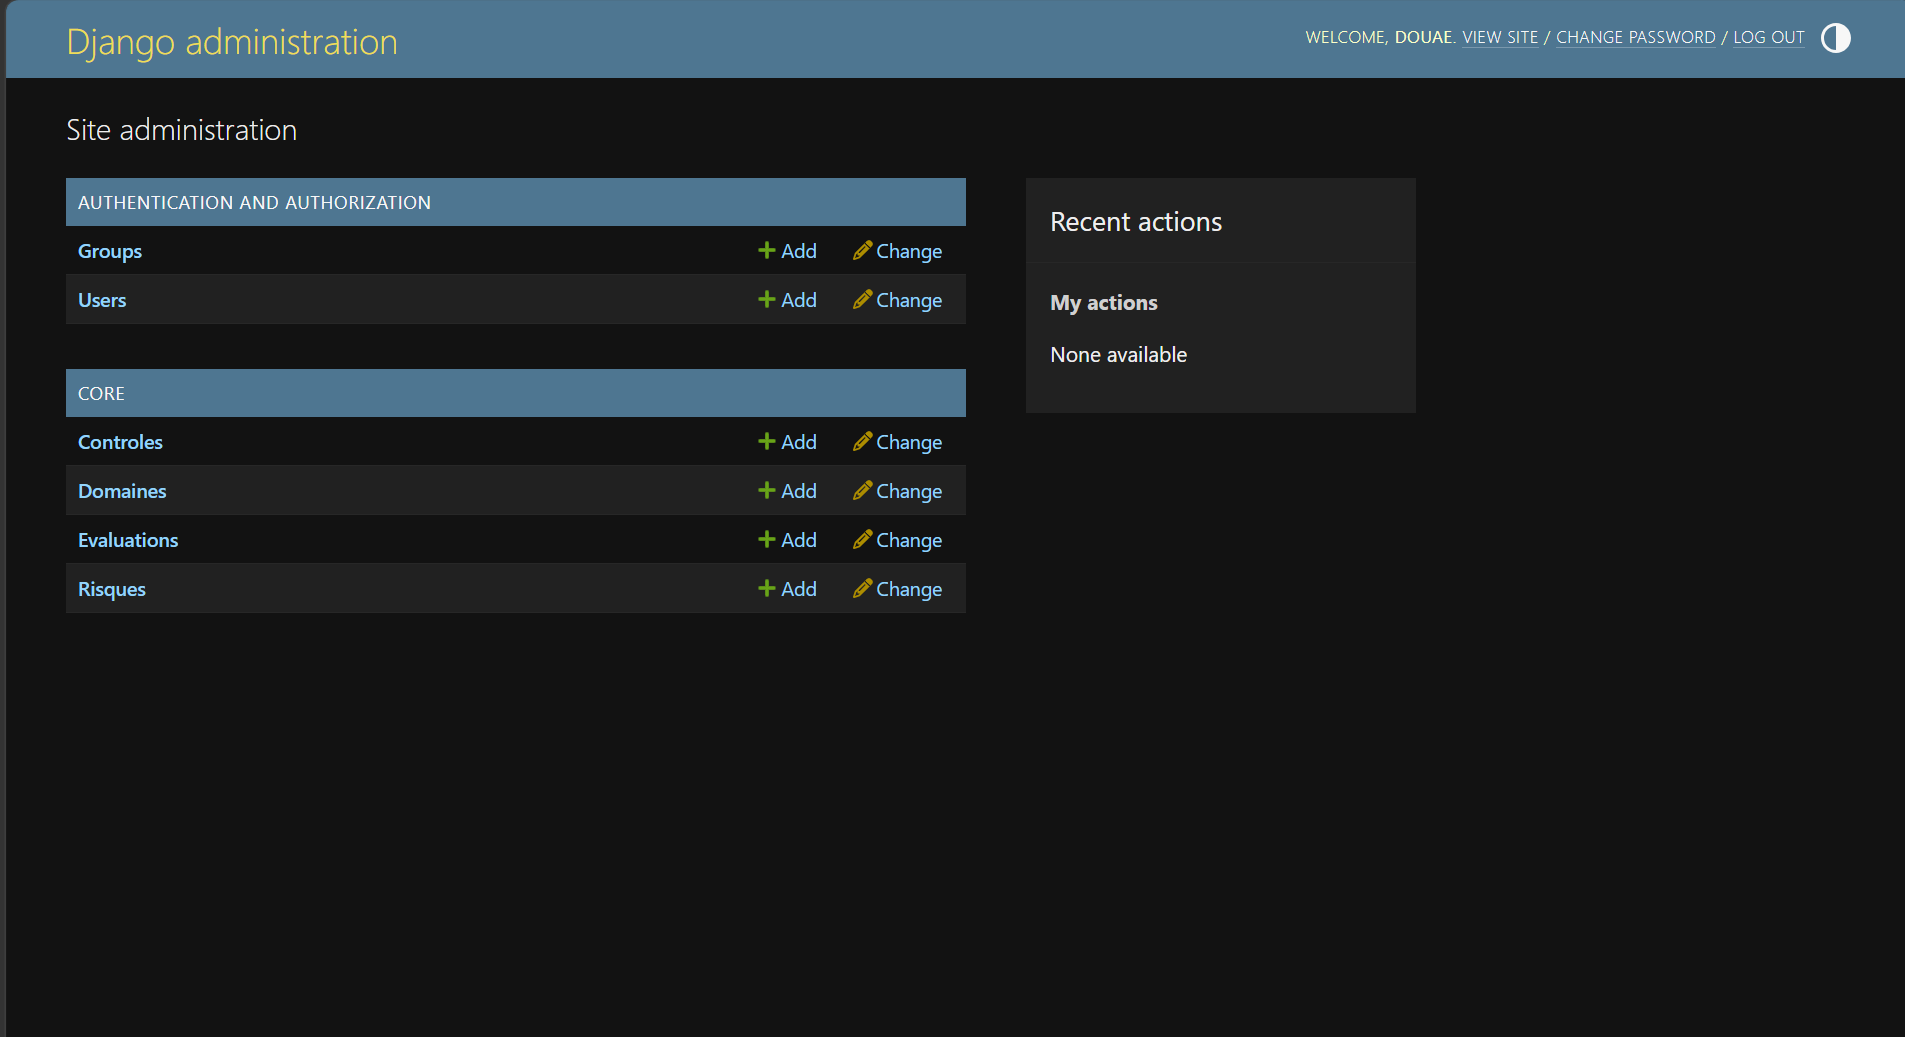
\includegraphics[width=0.85\linewidth]{01_admin_home_empty.png}
\caption{Admin Django avec l'application \code{core} (Controles, Domaines, Evaluations, Risques)}
\end{figure}

\subsection{Domaines et contrôles}
Les cinq domaines ont été créés en premier, puis les huit contrôles, chacun rattaché à son domaine.

\begin{figure}[H]
\centering
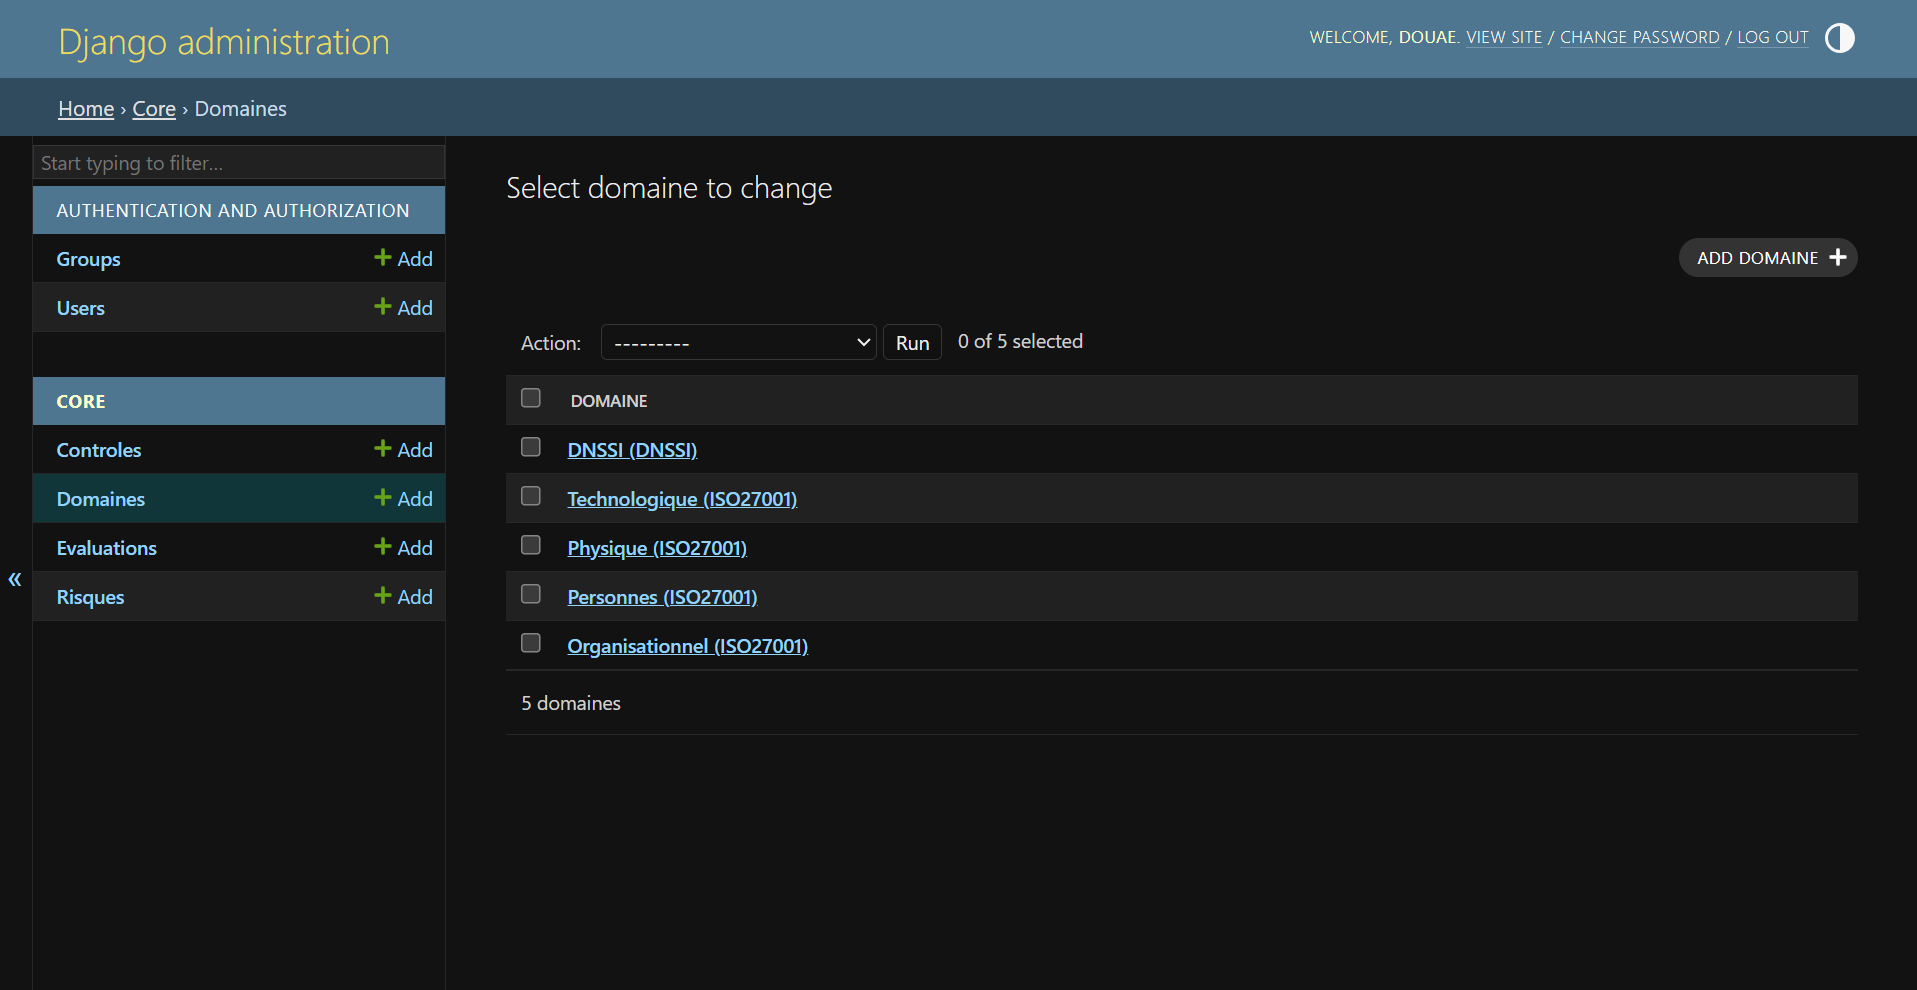
\includegraphics[width=0.85\linewidth]{06_admin_domains.png}
\caption{Les cinq domaines : quatre thèmes ISO 27001 et la DNSSI}
\end{figure}

\begin{figure}[H]
\centering
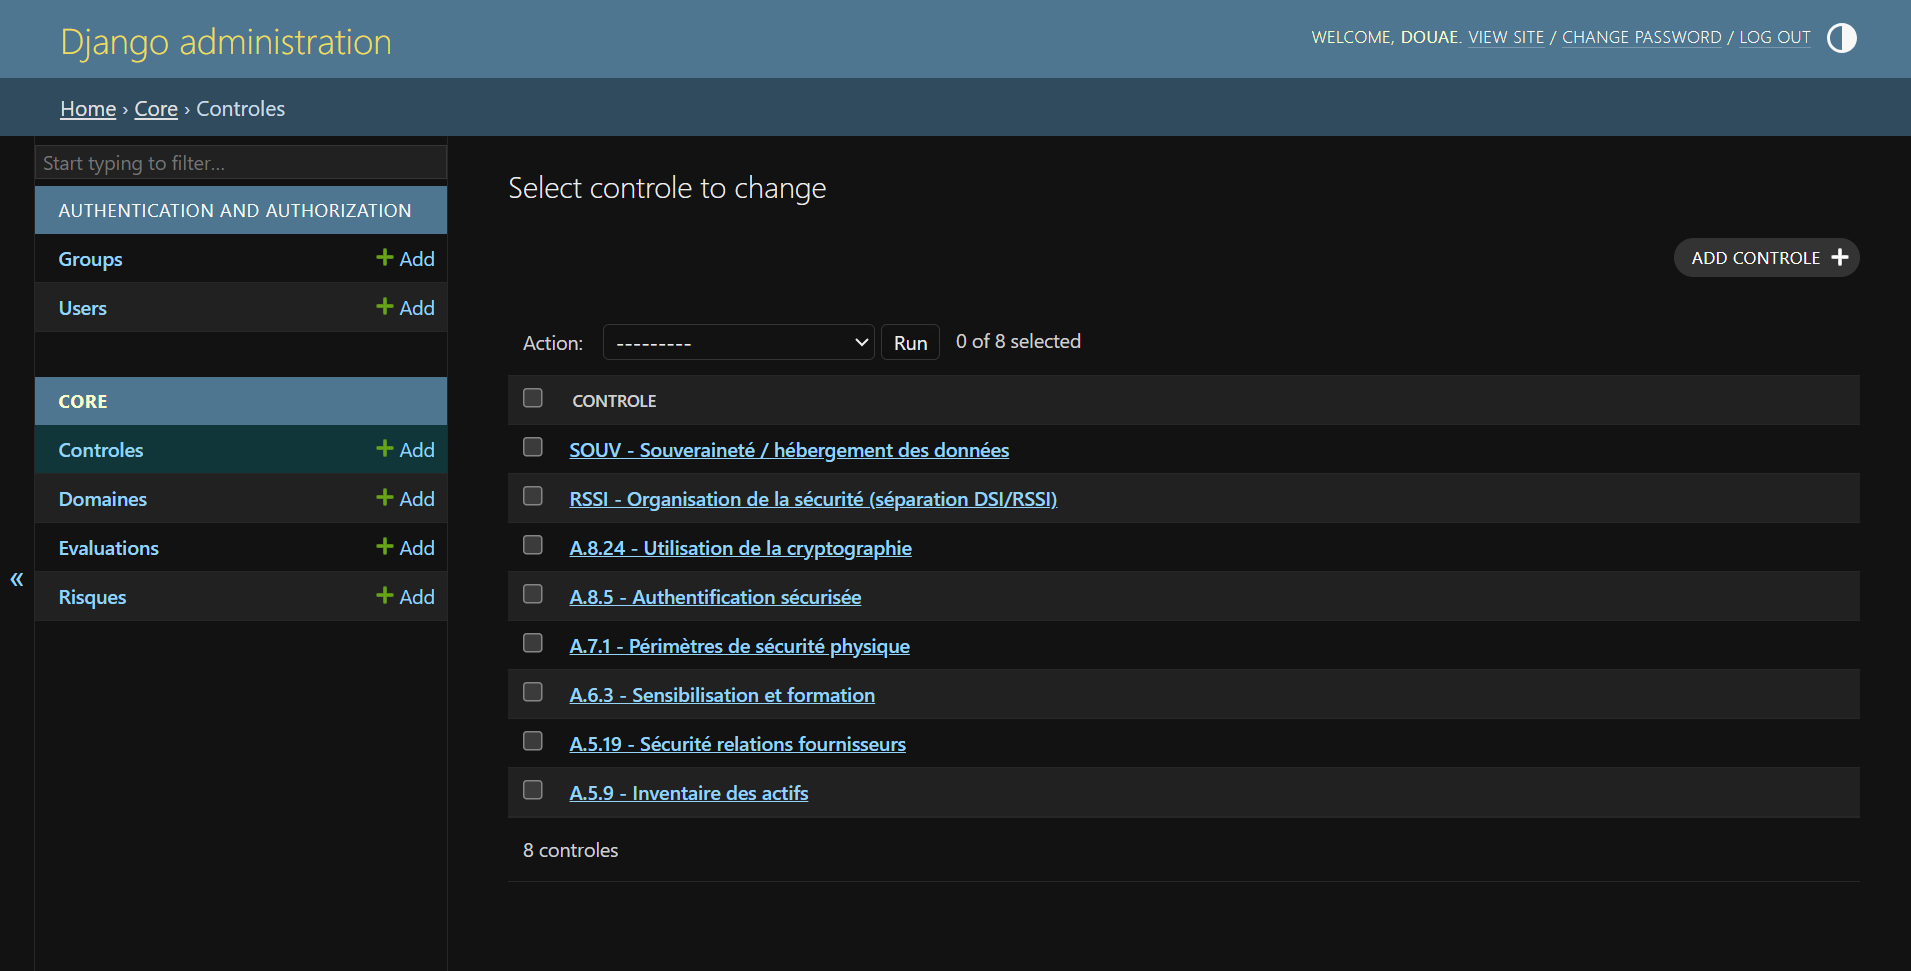
\includegraphics[width=0.85\linewidth]{05_admin_controls.png}
\caption{Les huit contrôles du catalogue AtlasPay}
\end{figure}

\subsection{Évaluations}
Une évaluation a été saisie par contrôle, avec son statut et un commentaire facultatif pour les preuves.

\begin{figure}[H]
\centering
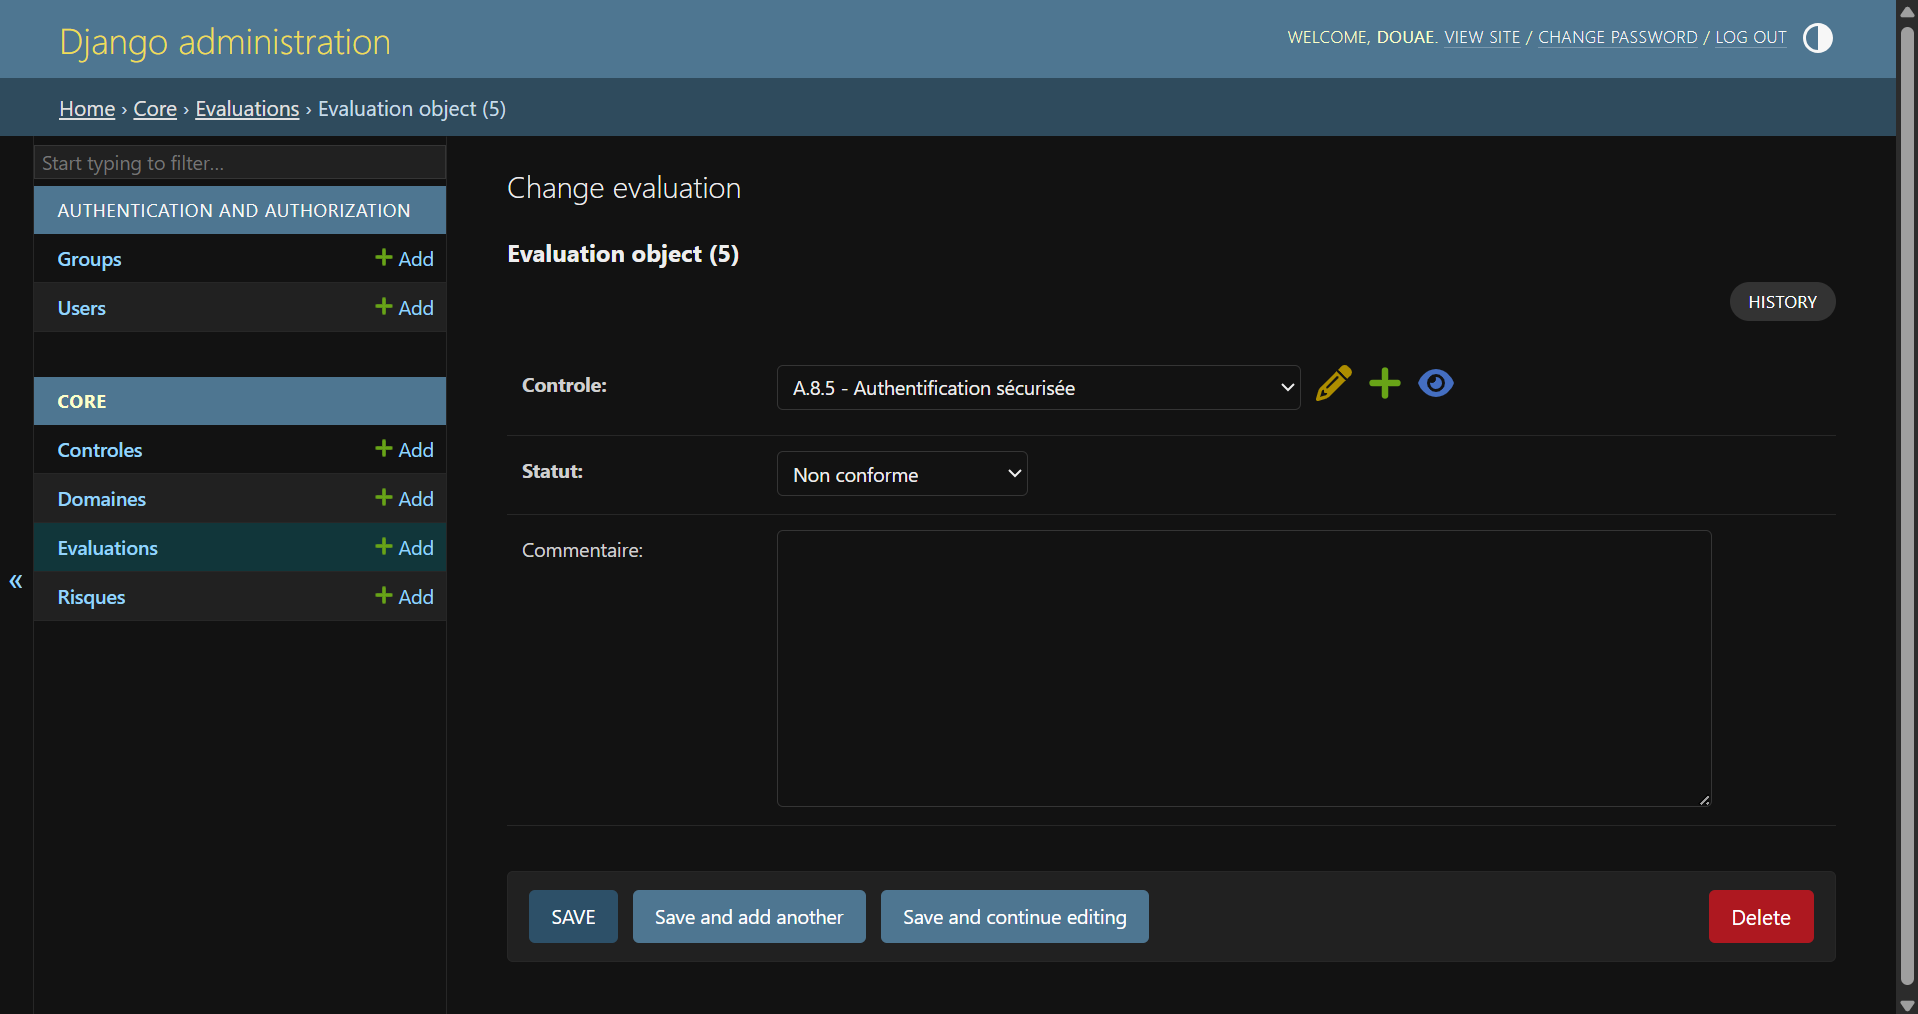
\includegraphics[width=0.85\linewidth]{08_evaluation_edit.png}
\caption{Évaluation d'A.8.5 Authentification sécurisée : \emph{Non conforme}}
\end{figure}

\begin{figure}[H]
\centering
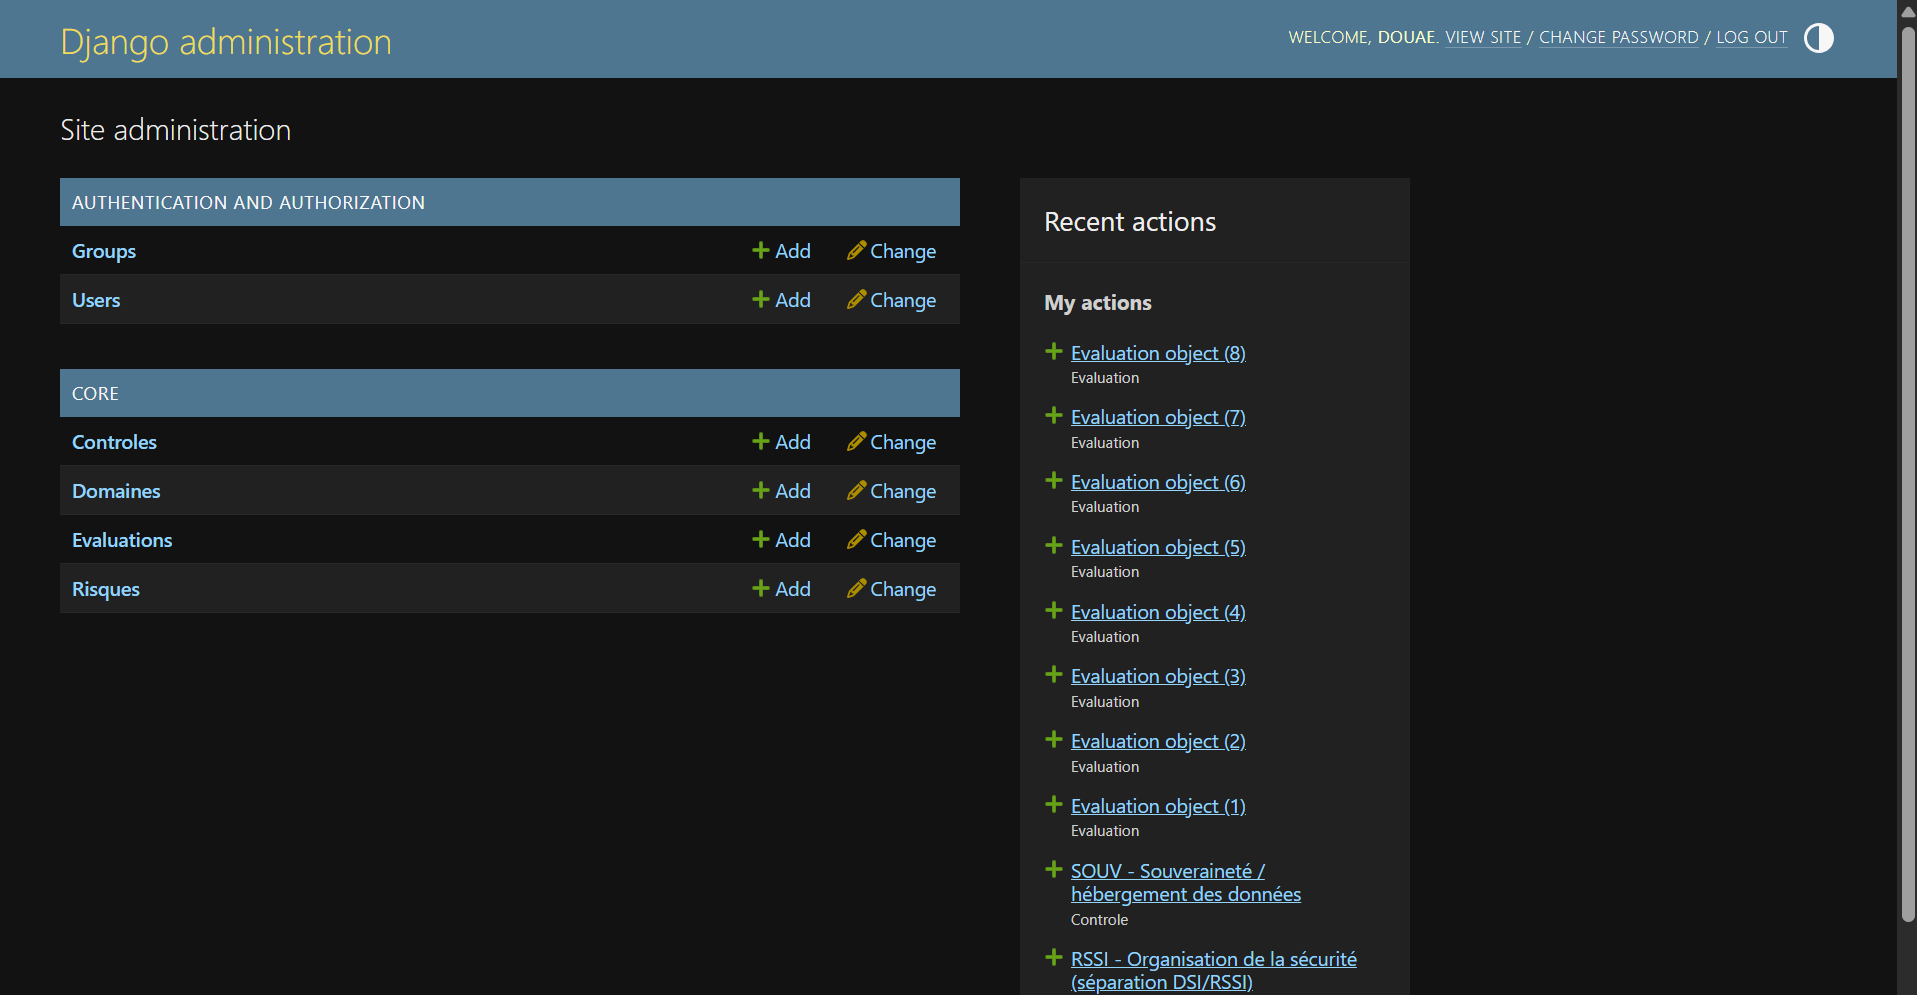
\includegraphics[width=0.85\linewidth]{03_admin_recent_actions.png}
\caption{Journal de l'admin montrant les contrôles et les huit évaluations créés}
\end{figure}

\subsection{Vérification dans le shell Django}
Avant de construire le dashboard, le calcul de conformité a été vérifié directement sur la base de données :

\begin{figure}[H]
\centering
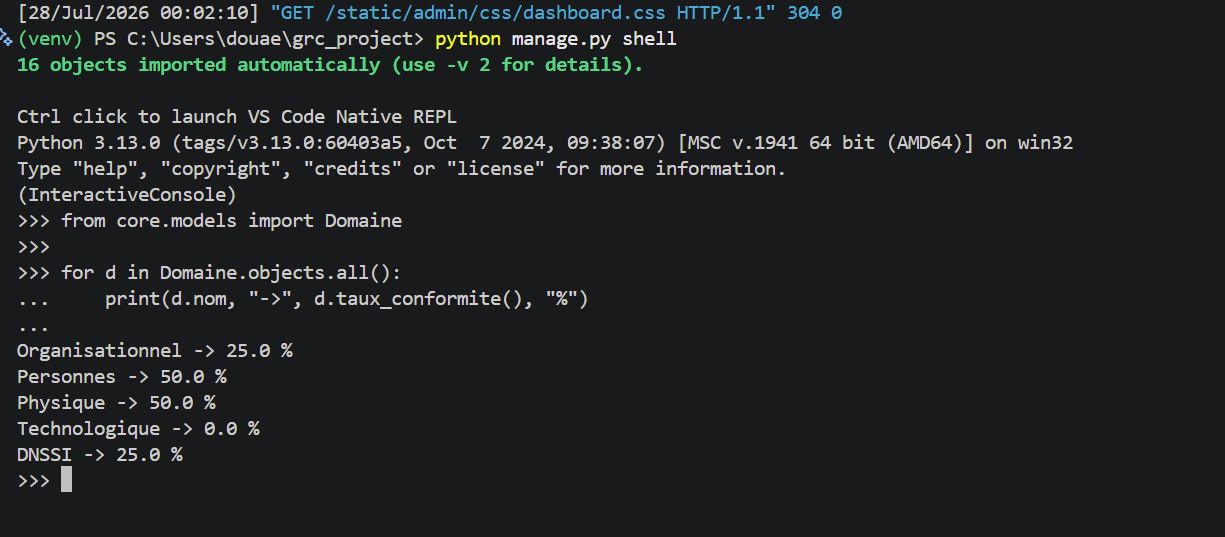
\includegraphics[width=0.75\linewidth]{02_shell_compliance_rates.png}
\caption{Taux de conformité par domaine calculé par \code{taux\_conformite()}}
\end{figure}

\subsection{Dashboard}
Le dashboard réunit les deux vues sur une seule page. Dans sa version finale, chaque page étend \code{base.html}, qui ajoute une barre de navigation, et le dashboard applique un code couleur : les taux sont classés \code{taux-bas} ($<30\,\%$), \code{taux-moyen} ($<70\,\%$) ou \code{taux-haut}, et chaque risque prend la classe de son niveau (\code{critique}, \code{élevé}, \ldots).

\begin{figure}[H]
\centering
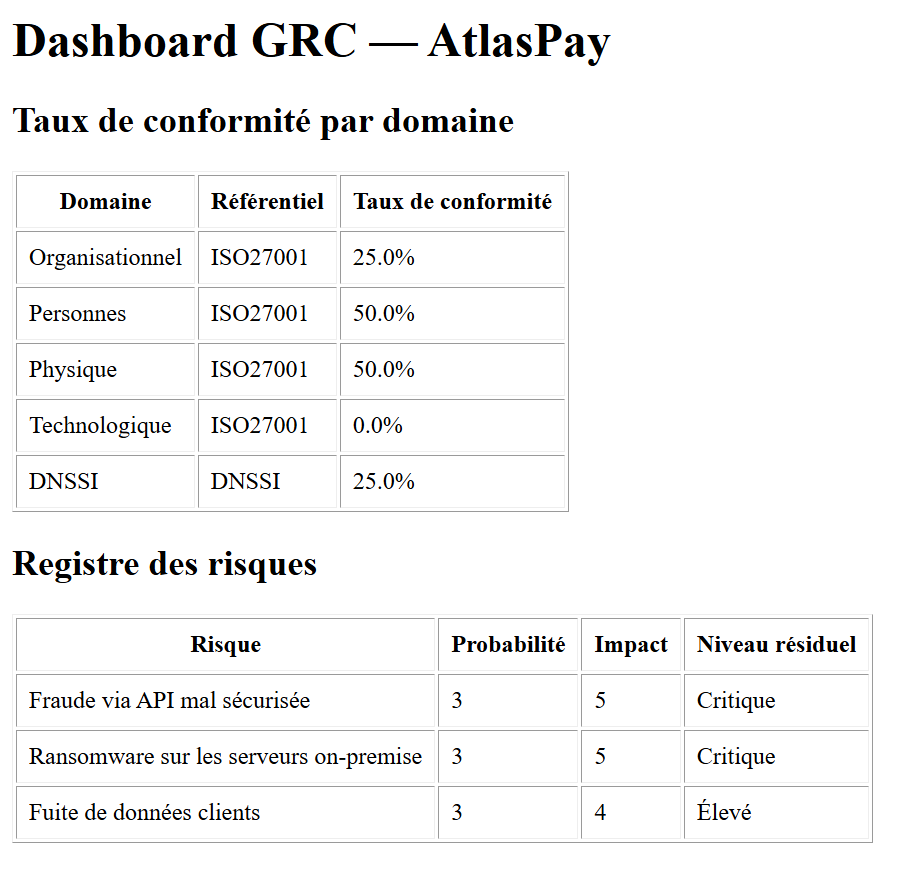
\includegraphics[width=0.6\linewidth]{09_dashboard.png}
\caption{Dashboard GRC d'AtlasPay (première version, avant le gabarit commun et la feuille de style)}
\end{figure}

% ================= 8 =================
\clearpage
\section{Résultats --- évaluation d'AtlasPay}
\subsection{Conformité par domaine}

\begin{figure}[H]
\centering
\begin{tikzpicture}
\begin{axis}[xbar,width=0.8\linewidth,height=5.5cm,xmin=0,xmax=100,
  symbolic y coords={DNSSI,Technologique,Physique,Personnes,Organisationnel},ytick=data,
  xlabel={Taux de conformité (\%)},nodes near coords,nodes near coords align={horizontal},
  every node near coord/.append style={font=\small,/pgf/number format/fixed zerofill,/pgf/number format/precision=1,/pgf/number format/use comma},
  bar width=11pt,enlarge y limits=0.15,xmajorgrids,grid style={black!15},
  y tick label style={font=\small},axis line style={black!40}]
\addplot[fill=accent,draw=none] coordinates {(25,Organisationnel) (50,Personnes) (50,Physique) (0,Technologique) (25,DNSSI)};
\end{axis}
\end{tikzpicture}
\caption{Taux de conformité par domaine}
\end{figure}

\begin{table}[H]
\centering\small
\begin{tabular}{@{}llllr@{}}
\toprule
\textbf{Domaine} & \textbf{Contrôle} & \textbf{Statut} & \textbf{Date} & \textbf{Taux}\\
\midrule
\multirow{2}{*}{Organisationnel} & A.5.9 & partiel & 27/07/2026 & \multirow{2}{*}{25,0\,\%}\\
 & A.5.19 & non conforme & 27/07/2026 & \\
Personnes & A.6.3 & partiel & 27/07/2026 & 50,0\,\%\\
Physique & A.7.1 & partiel & 27/07/2026 & 50,0\,\%\\
\multirow{2}{*}{Technologique} & A.8.5 & non conforme & 28/07/2026 & \multirow{2}{*}{0,0\,\%}\\
 & A.8.24 & non conforme & 28/07/2026 & \\
\multirow{2}{*}{DNSSI} & RSSI & partiel & 28/07/2026 & \multirow{2}{*}{25,0\,\%}\\
 & SOUV & non conforme & 28/07/2026 & \\
\bottomrule
\end{tabular}
\caption{Détail des évaluations (issu de la base de données du projet)}
\end{table}

\subsection{Registre des risques}
\begin{table}[H]
\centering\small
\begin{tabularx}{\linewidth}{@{}lXcccll@{}}
\toprule
\textbf{N°} & \textbf{Risque} & \textbf{P} & \textbf{I} & \textbf{S} & \textbf{Niveau} & \textbf{Contrôles liés}\\
\midrule
R1 & Fraude via API mal sécurisée & 3 & 5 & 15 & \lvl{rcrit}{Critique} & A.8.5\\
R2 & Ransomware sur les serveurs on-premise & 3 & 5 & 15 & \lvl{rcrit}{Critique} & A.7.1, A.8.24\\
R3 & Fuite de données clients & 3 & 4 & 12 & \lvl{rhigh}{Élevé} & A.5.19\\
\bottomrule
\end{tabularx}
\caption{Registre des risques et correspondance risques--contrôles}
\end{table}

\subsection{Analyse}
\begin{itemize}
  \item \textbf{Aucun risque n'est couvert par un contrôle conforme.} R1 dépend d'A.8.5 (non conforme), R2 d'A.7.1 (partiel) et d'A.8.24 (non conforme), R3 d'A.5.19 (non conforme). Le registre et les évaluations racontent la même histoire.
  \item \textbf{La technologie est l'écart critique.} À 0\,\%, le domaine Technologique porte les contrôles des deux risques critiques : authentification forte sur les API de paiement (MFA, gestion des jetons) et chiffrement des données au repos et en transit.
  \item \textbf{La gouvernance est fragile.} Avec 25\,\%, le domaine Organisationnel révèle un inventaire des actifs incomplet et l'absence de sécurité formalisée avec les fournisseurs --- seul contrôle relié au risque de fuite de données clients.
  \item \textbf{Exposition réglementaire DNSSI.} Une séparation DSI/RSSI partielle et un hébergement des données non conforme constituent un écart réglementaire direct pour un acteur marocain du paiement.
\end{itemize}

\begin{keybox}[title=Ordre de remédiation recommandé]
\begin{enumerate}[leftmargin=*,label=\arabic*.]
  \item A.8.5 Authentification sécurisée --- réduit R1 (critique).
  \item A.8.24 Cryptographie --- réduit R2 (critique) et protège aussi les données concernées par R3.
  \item A.5.19 Sécurité fournisseurs --- seul contrôle relié à R3.
  \item A.7.1 Périmètres physiques --- complète la couverture de R2 sur les serveurs internes.
  \item SOUV et RSSI --- comblent les écarts réglementaires DNSSI.
\end{enumerate}
\end{keybox}

% ================= 9 =================
\section{Tests et validation}
Une suite de tests automatisés (\code{core/tests.py}) rend les règles de calcul vérifiables. Elle s'exécute avec \code{python manage.py test} et passe 8 tests sur 8.

\begin{table}[H]
\centering\small
\begin{tabularx}{\linewidth}{@{}lX@{}}
\toprule
\textbf{Test} & \textbf{Vérifie que}\\
\midrule
\code{test\_sans\_evaluation\_retourne\_none} & Sans évaluation $\Rightarrow$ \code{None}, pas 0\,\%\\
\code{test\_ponderation} & $(1+0{,}5+0)/3 = 50\,\%$\\
\code{test\_non\_applicable\_exclu} & N/A est exclu du dénominateur\\
\code{test\_seulement\_na\_retourne\_none} & Uniquement N/A $\Rightarrow$ \code{None}\\
\code{test\_seuils} & Tous les seuils de niveau de risque\\
\code{test\_pages\_repondent} & Les quatre pages répondent HTTP 200\\
\code{test\_ajout\_risque\_redirige\_vers\_dashboard} & Un risque valide est enregistré puis redirigé\\
\code{test\_dashboard\_reproduit\_les\_taux\_documentes} & Les données de démo reproduisent les taux documentés\\
\bottomrule
\end{tabularx}
\caption{Suite de tests}
\end{table}

La commande \code{python manage.py seed\_demo} recrée le jeu de données AtlasPay à partir de la base d'origine (statuts et liens avec les risques), afin que toute personne clonant le dépôt obtienne le même dashboard. Elle est idempotente et accepte l'option \code{--reset}.

% ================= 10 =================
\section{Revue de sécurité et de qualité}
S'agissant d'un outil de sécurité, l'application doit elle-même respecter les bonnes pratiques. Le code et la base de données du projet ont été revus avant publication.

\begin{table}[H]
\centering\small
\begin{tabularx}{\linewidth}{@{}lXll@{}}
\toprule
\textbf{N°} & \textbf{Constat} & \textbf{Gravité} & \textbf{Statut}\\
\midrule
S1 & \code{SECRET\_KEY} écrite en dur dans les paramètres & Élevée & Corrigé --- variable d'env.\\
S2 & \code{DEBUG = True} écrit en dur & Moyenne & Corrigé --- variable d'env.\\
S3 & \code{ALLOWED\_HOSTS} non paramétrable & Faible & Corrigé --- variable d'env.\\
S4 & Base de données (hash du mot de passe admin, e-mail) dans le dossier du projet & Moyenne & Corrigé --- \code{.gitignore}\\
S5 & Pages applicatives accessibles sans authentification & Moyenne & Ouvert --- feuille de route\\
S6 & \code{probabilite}/\code{impact} acceptent n'importe quel entier & Faible & Ouvert --- feuille de route\\
Q1 & Contrôle A.8.24 en double dans la base (second enregistrement sans évaluation, relié à R2) & Faible & Ouvert --- feuille de route\\
\bottomrule
\end{tabularx}
\caption{Constats}
\end{table}

Le constat Q1 montre l'intérêt d'une contrainte d'unicité sur \code{Controle.code} : le doublon n'a pas d'évaluation et n'entre donc pas dans le taux de conformité, mais il apparaît comme contrôle de traitement de R2.

Protections déjà actives grâce au framework : jetons CSRF sur chaque formulaire, protection contre le clickjacking (\code{X-Frame-Options: DENY}), requêtes paramétrées par l'ORM (pas de surface d'injection SQL dans le code applicatif), échappement automatique des templates (XSS) et validateurs de mots de passe pour les comptes admin.

% ================= 11 =================
\section{Limites et feuille de route}
\begin{table}[H]
\centering\small
\begin{tabularx}{\linewidth}{@{}XX@{}}
\toprule
\textbf{Limite} & \textbf{Amélioration prévue}\\
\midrule
Le \og niveau résiduel \fg{} n'utilise que $P\times I$ : c'est en réalité le risque \emph{inhérent} & Réduire le score selon la conformité des contrôles liés\\
Pas de contrôle d'accès sur les vues applicatives & \code{@login\_required}, rôles (auditeur, propriétaire du risque, lecture seule)\\
Probabilité et impact non bornés & \code{MinValueValidator(1)}, \code{MaxValueValidator(5)}\\
Codes de contrôle en double possibles & \code{unique=True} sur \code{Controle.code}\\
Le taux compte toutes les évaluations, pas la dernière par contrôle & Dernière évaluation par contrôle, historique et tendances\\
Un taux \code{None} s'affiche \og None\% \fg{} sur le dashboard & Afficher \og N/A \fg{} pour les domaines non évalués\\
Évaluations affichées \og Evaluation object (n) \fg{} dans l'admin & \code{\_\_str\_\_}, \code{list\_display}, filtres\\
Catalogue partiel (8 contrôles) & Annexe~A complète (93 contrôles) et import DNSSI\\
\bottomrule
\end{tabularx}
\caption{Limites et feuille de route}
\end{table}

% ================= 12 =================
\section{Guide d'installation}
Prérequis : Python 3.12 ou plus récent et Git.
\begin{lstlisting}[language=bash]
git clone https://github.com/Dorvae/grc-compliance-tool.git
cd grc-compliance-tool
python -m venv venv
venv\Scripts\activate          # Linux/macOS : source venv/bin/activate
pip install -r requirements.txt
python manage.py migrate
python manage.py seed_demo       # données de démonstration (optionnel)
python manage.py createsuperuser
python manage.py runserver
\end{lstlisting}
Le dashboard est alors disponible à l'adresse \code{http://127.0.0.1:8000/dashboard/} et le back-office à \code{/admin/}. En dehors du développement local, renseigner les variables de \code{.env.example} avec une nouvelle clé secrète aléatoire et \code{DJANGO\_DEBUG=False}.

% ================= 13 =================
\section{Conclusion}
Le projet livre un outil GRC fonctionnel qui transforme une liste de contrôles de sécurité en indicateurs de conformité mesurables et les relie aux risques métier. Appliqué à AtlasPay, il montre sur une seule page que les contrôles technologiques constituent le point faible et qu'ils sous-tendent les deux risques critiques --- exactement le type de priorisation fondée sur des preuves dont les équipes d'audit et de risques ont besoin. Le code est compact, testé et structuré pour que les éléments de la feuille de route puissent être ajoutés progressivement.

\clearpage
\appendix
\section{Structure du dépôt}
\begin{lstlisting}
grc-compliance-tool/
|-- README.md  LICENSE  requirements.txt  .env.example  .gitignore
|-- manage.py
|-- grc_project/   settings.py  urls.py  wsgi.py  asgi.py
|-- core/          models.py  views.py  forms.py  admin.py  tests.py
|   |-- templates/        base, home, dashboard, 2 formulaires
|   |-- static/core/      style.css
|   |-- migrations/       0001_initial.py
|   `-- management/commands/seed_demo.py
`-- docs/
    |-- GRC_Tool_Documentation.pdf
    |-- latex/            source LaTeX de ce document
    `-- screenshots/
\end{lstlisting}

\end{document}
